\chapter{Diseño}
\title{Diseño}
\label{cap:Diseno}

\section{Arquitectura}
Como se ha ido viendo en los capítulos anteriores, el dispositivo que se desea desarrollar
tiene que hacer la función básica del director de la banda de música durante una actuación,
es decir, marcar el mismo pulso a los músicos.\\

Si recordamos el esquema planteado en la figura \ref{fig:modeladoconceptual} y todo lo
que se ha ido desarrollando a través de los capítulos anteriores, podemos decir
que el sistema sigue una arquitectura de repositorio -o pizarra- (siendo el repositorio activo):

\begin{itemize}
  \item El director es el centro de todo. Se encarga de realizar la comunicación con los músicos
  \item Los músicos son subsistemas independientes (aunque tengan que estar sincronizados)
  \item Alto acoplamiento entre los músicos y el director
\end{itemize}

A parte de la relación existente entre músicos y director, no debemos olvidar que
deseamos comunicarnos desde un dispositivo (Android según las especificaciones pero que,
como se verá en la implementación, valdrá cualquier SO). Es por ello que el diagrama
de despliegue queda como en la figura \ref{fig:diagramadespliegue}.\\

\section{Diagrama conceptual}
\title{Diagrama conceptual}
Este diagrama (que podemos ver en la figura \ref{fig:modeloconceptual})
nos da una idea de cómo se encuentran interrelacionados los diferentes
agentes del sistema. En nuestro caso, podemos ver cómo un ``Director" está asociado
a muchos ``Músicos" (o ninguno) y un ``Músico" solo tiene asignado un director.\\


\begin{figure}[!htb]
\centering
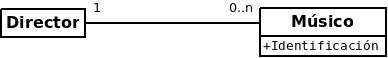
\includegraphics[width=1\textwidth]{./imagenes/modeloconceptual}
\caption{Modelo conceptual} \label{fig:modeloconceptual}
\end{figure}

\begin{figure}[htb]
\centering
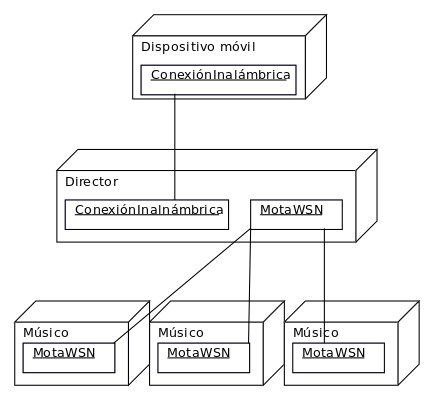
\includegraphics[width=1\textwidth]{./imagenes/diagramadespliegue}
\caption{Diagrama de despliegue} \label{fig:diagramadespliegue}
\end{figure}

\section{Diagrama de secuencia del sistema}
Para ver desde otra perspectiva el funcionamiento del sistema, se ha creado el diagrama
de secuencia de la figura \ref{fig:diagramasecuencia}\\


\begin{figure}[!htb]
\centering
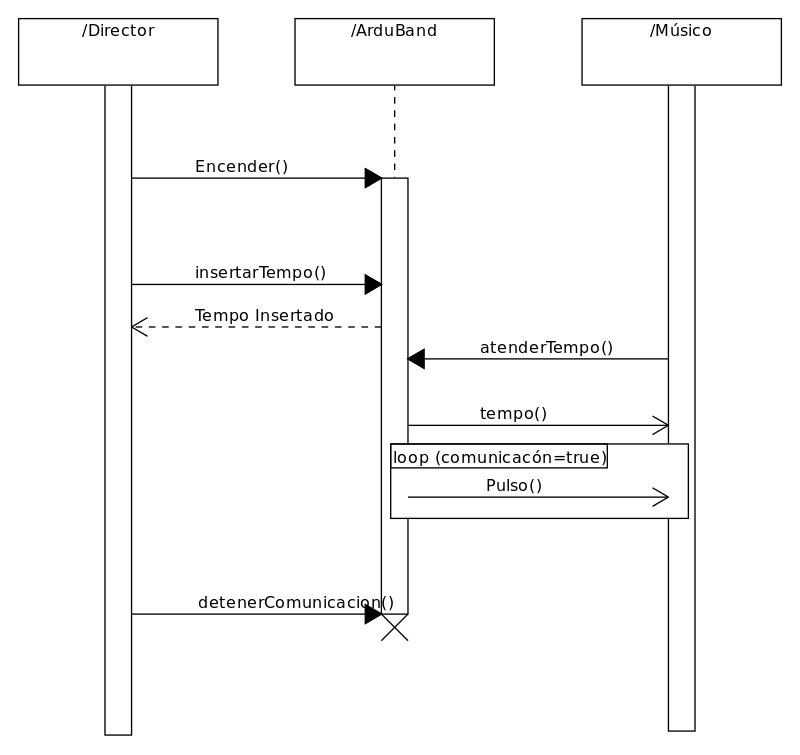
\includegraphics[width=1\textwidth]{./imagenes/diagramasecuencia}
\caption{Diagrama de secuencia} \label{fig:diagramasecuencia}
\end{figure}


\section{Diagramas de comunicación}
\title{Diagramas de comunicación}

Estos diagramas permiten conocer la relación que hay entre los distintos
conceptos del sistema y qué información pasa de unos a otros.\\

Los casos de uso expuestos en \ref{subsec:casosdeuso} se han diseñado según
se muestra en las figuras \ref{fig:comunicacion1},  \ref{fig:comunicacion2} y
\ref{fig:comunicacion3}.\\

\begin{figure}[htb]
\centering
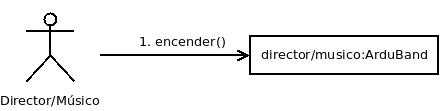
\includegraphics[width=1\textwidth]{./imagenes/comunicacion1}
\caption{Diagrama de comunicación 1} \label{fig:comunicacion1}
\end{figure}

\begin{figure}[htb]
\centering
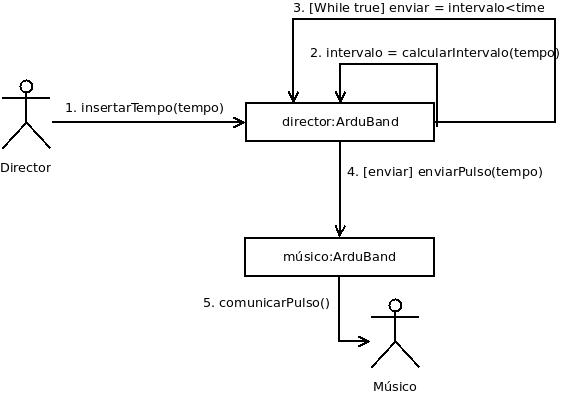
\includegraphics[width=1\textwidth]{./imagenes/comunicacion2}
\caption{Diagrama de comunicación 2} \label{fig:comunicacion2}
\end{figure}

\begin{figure}[htb]
\centering
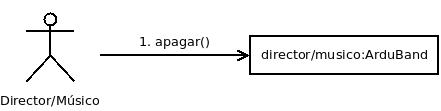
\includegraphics[width=1\textwidth]{./imagenes/comunicacion3}
\caption{Diagrama de comunicación 3} \label{fig:comunicacion3}
\end{figure}

\section{Interfaces}
\title{Interfaces}

Como medio de interacción entre el director y el dispositivo, se va a utilizar,
como se ha venido hablando a lo largo de la memoria, un dispositivo Android y/o
Android Wear. En la implementación se verá exactamente qué sistema utilizar
para realizar la comunicación.\\

En cuanto a la interfaz entre el dispositivo y el músico, ya se mencionaba en
los primeros capítulos de esta memoria la intención de utilizar algún actuador
para avisar al músico. Ya que no se quiere que sea algo muy llamativo, se optará
por un micromotor vibrador (en la implementación se elegirá cuál).\\


\subsection{Interfaz músico-sistema}
\title{Interfaz músico-sistema}
\begin{figure}[!htb]
\centering
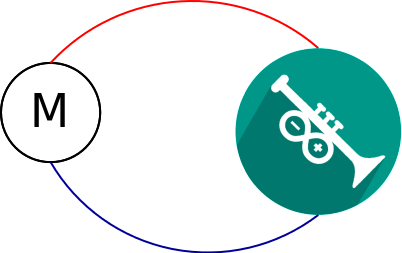
\includegraphics[width=1\textwidth]{./imagenes/motorarduband}
\caption{Interfaz músico-sistema} \label{fig:motorarduband}
\end{figure}

\subsection{Interfaces gráficas}
\title{Interfaces gráficas}

Corresponde con la interfaz director-sistema.\\

\begin{figure}[htb]
\centering
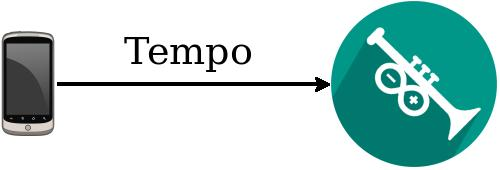
\includegraphics[width=1\textwidth]{./imagenes/movilarduband}
\caption{Esquema de comunicación entre el dispositivo móvil y ArduBand} \label{fig:movilarduband}
\end{figure}

El esquema que se desea seguir es el de la figura \ref{fig:movilarduband}.

Con objeto de tener una guía para de cara a la implementación, se ha planteado un
prototipo del diseño de la interfaz gráfica que se puede ver en la figura
\ref{fig:prototipointerfaz} (realizado con el software \href{http://pencil.evolus.vn/}{Pencil}).\\

\begin{figure}[htb]
\centering
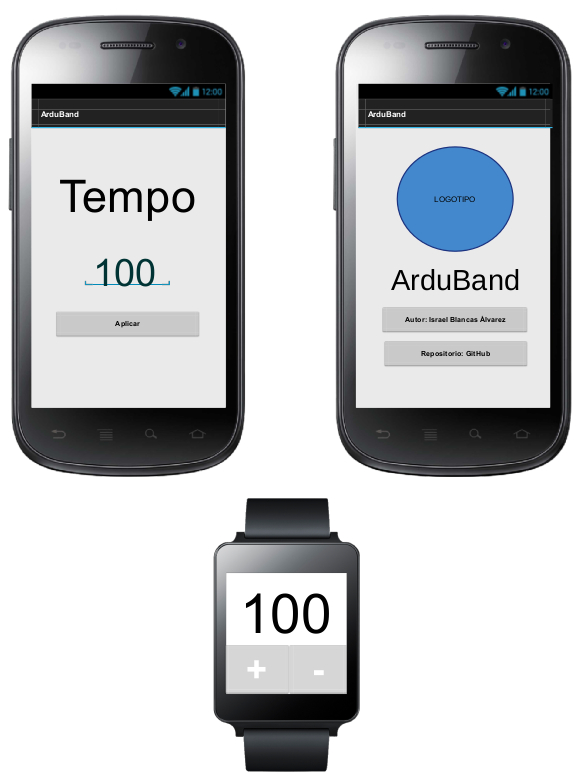
\includegraphics[width=1\textwidth]{./imagenes/prototipointerfaz}
\caption{Prototipo de interfaz} \label{fig:prototipointerfaz}
\end{figure}

En la figura \ref{fig:prototipointerfaz} podemos observar tres pantallas (dos de de ellas
pertenecientes a teléfono móvil y una tercera a un reloj Android Wear).

\begin{description}
  \item[Android] \hfill \\
    Se ha buscado que sea una interfaz lo más simple posible para que el usuario no dude
    en su uso. En el centro se ha insertado un campo para que se añada el tempo y un botón de aplicar.
    Se ha añadido una sección ``Sobre" en el que se han colocado dos enlaces (que
    llevan a la web del autor y al repositorio del proyecto) y el logotipo de la aplicación
  \item[Android Wear] \hfill \\
    Más sencilla que la anterior. En grande se muestra el tempo. Hay dos botones en la parte inferior que permiten
    aumentar o disminuir la cifra de tempo. Cuando se desee aplicar, se pulsa encima del tempo y el sistema
    comienza a funciona
\end{description}

Cuando se realice la implementación, se tratará de seguir lo más fielmente posible las directrices de diseño que
Google da en su guía para desarrolladores (Material Design) \cite{googlematerial}.
